% Options for packages loaded elsewhere
\PassOptionsToPackage{unicode}{hyperref}
\PassOptionsToPackage{hyphens}{url}
\PassOptionsToPackage{dvipsnames,svgnames,x11names}{xcolor}
%
\documentclass[
  letterpaper,
  DIV=11,
  numbers=noendperiod]{scrartcl}

\usepackage{amsmath,amssymb}
\usepackage{lmodern}
\usepackage{iftex}
\ifPDFTeX
  \usepackage[T1]{fontenc}
  \usepackage[utf8]{inputenc}
  \usepackage{textcomp} % provide euro and other symbols
\else % if luatex or xetex
  \usepackage{unicode-math}
  \defaultfontfeatures{Scale=MatchLowercase}
  \defaultfontfeatures[\rmfamily]{Ligatures=TeX,Scale=1}
\fi
% Use upquote if available, for straight quotes in verbatim environments
\IfFileExists{upquote.sty}{\usepackage{upquote}}{}
\IfFileExists{microtype.sty}{% use microtype if available
  \usepackage[]{microtype}
  \UseMicrotypeSet[protrusion]{basicmath} % disable protrusion for tt fonts
}{}
\makeatletter
\@ifundefined{KOMAClassName}{% if non-KOMA class
  \IfFileExists{parskip.sty}{%
    \usepackage{parskip}
  }{% else
    \setlength{\parindent}{0pt}
    \setlength{\parskip}{6pt plus 2pt minus 1pt}}
}{% if KOMA class
  \KOMAoptions{parskip=half}}
\makeatother
\usepackage{xcolor}
\setlength{\emergencystretch}{3em} % prevent overfull lines
\setcounter{secnumdepth}{-\maxdimen} % remove section numbering
% Make \paragraph and \subparagraph free-standing
\ifx\paragraph\undefined\else
  \let\oldparagraph\paragraph
  \renewcommand{\paragraph}[1]{\oldparagraph{#1}\mbox{}}
\fi
\ifx\subparagraph\undefined\else
  \let\oldsubparagraph\subparagraph
  \renewcommand{\subparagraph}[1]{\oldsubparagraph{#1}\mbox{}}
\fi


\providecommand{\tightlist}{%
  \setlength{\itemsep}{0pt}\setlength{\parskip}{0pt}}\usepackage{longtable,booktabs,array}
\usepackage{calc} % for calculating minipage widths
% Correct order of tables after \paragraph or \subparagraph
\usepackage{etoolbox}
\makeatletter
\patchcmd\longtable{\par}{\if@noskipsec\mbox{}\fi\par}{}{}
\makeatother
% Allow footnotes in longtable head/foot
\IfFileExists{footnotehyper.sty}{\usepackage{footnotehyper}}{\usepackage{footnote}}
\makesavenoteenv{longtable}
\usepackage{graphicx}
\makeatletter
\def\maxwidth{\ifdim\Gin@nat@width>\linewidth\linewidth\else\Gin@nat@width\fi}
\def\maxheight{\ifdim\Gin@nat@height>\textheight\textheight\else\Gin@nat@height\fi}
\makeatother
% Scale images if necessary, so that they will not overflow the page
% margins by default, and it is still possible to overwrite the defaults
% using explicit options in \includegraphics[width, height, ...]{}
\setkeys{Gin}{width=\maxwidth,height=\maxheight,keepaspectratio}
% Set default figure placement to htbp
\makeatletter
\def\fps@figure{htbp}
\makeatother

\KOMAoption{captions}{tableheading}
\makeatletter
\makeatother
\makeatletter
\makeatother
\makeatletter
\@ifpackageloaded{caption}{}{\usepackage{caption}}
\AtBeginDocument{%
\ifdefined\contentsname
  \renewcommand*\contentsname{Table of contents}
\else
  \newcommand\contentsname{Table of contents}
\fi
\ifdefined\listfigurename
  \renewcommand*\listfigurename{List of Figures}
\else
  \newcommand\listfigurename{List of Figures}
\fi
\ifdefined\listtablename
  \renewcommand*\listtablename{List of Tables}
\else
  \newcommand\listtablename{List of Tables}
\fi
\ifdefined\figurename
  \renewcommand*\figurename{Figure}
\else
  \newcommand\figurename{Figure}
\fi
\ifdefined\tablename
  \renewcommand*\tablename{Table}
\else
  \newcommand\tablename{Table}
\fi
}
\@ifpackageloaded{float}{}{\usepackage{float}}
\floatstyle{ruled}
\@ifundefined{c@chapter}{\newfloat{codelisting}{h}{lop}}{\newfloat{codelisting}{h}{lop}[chapter]}
\floatname{codelisting}{Listing}
\newcommand*\listoflistings{\listof{codelisting}{List of Listings}}
\makeatother
\makeatletter
\@ifpackageloaded{caption}{}{\usepackage{caption}}
\@ifpackageloaded{subcaption}{}{\usepackage{subcaption}}
\makeatother
\makeatletter
\@ifpackageloaded{tcolorbox}{}{\usepackage[many]{tcolorbox}}
\makeatother
\makeatletter
\@ifundefined{shadecolor}{\definecolor{shadecolor}{rgb}{.97, .97, .97}}
\makeatother
\makeatletter
\makeatother
\ifLuaTeX
  \usepackage{selnolig}  % disable illegal ligatures
\fi
\IfFileExists{bookmark.sty}{\usepackage{bookmark}}{\usepackage{hyperref}}
\IfFileExists{xurl.sty}{\usepackage{xurl}}{} % add URL line breaks if available
\urlstyle{same} % disable monospaced font for URLs
\hypersetup{
  pdftitle={An Ecologist's Guide to BIIGLE},
  colorlinks=true,
  linkcolor={blue},
  filecolor={Maroon},
  citecolor={Blue},
  urlcolor={Blue},
  pdfcreator={LaTeX via pandoc}}

\title{An Ecologist's Guide to BIIGLE}
\author{}
\date{}

\begin{document}
\maketitle
\ifdefined\Shaded\renewenvironment{Shaded}{\begin{tcolorbox}[breakable, boxrule=0pt, sharp corners, enhanced, borderline west={3pt}{0pt}{shadecolor}, frame hidden, interior hidden]}{\end{tcolorbox}}\fi

This is the living version of the document where users can suggest edits
to improve the Ecologist's Guide to BIIGLE. You can find the finalised,
origianl version on Zenodo here: LINK

\hypertarget{introduction}{%
\section{Introduction}\label{introduction}}

Hello and welcome to our BIIGLE manual. This document is intended to
help ecologists get started using BIIGLE to annotate their image and
video data. The manual was originally written to support new members of
the Deep-Sea Conservation Research Unit as well as undergraduate
students at the University of Plymouth. It is a collection of
information that we have found helpful to document in our experience of
setting up and using BIIGLE. It is not intended as a replacement for the
official BIIGLE manual available here https://biigle.de/manual. We
intend this to be a living document that others can contribute to here
https://github.com/DeepSeaCRU/CRU-resources. It is fair to say our
current instruction manual is bias toward image data (although video is
included), and only provides instructions for setting up using Amazon
Web Service as the host for your imagery. If you can provide instruction
for setting up on other cloud services, please contribute. But first
things first, you need to create a BIIGLE account. To create an account,
click on the ``sign up'' button in the top right corner of the website
(https://biigle.de/) homepage. Fill in the module with your details and
affiliation, choose a password and, after agreeing to the privacy notice
and the terms of use, click on sign up. To log in, click on the green
``login'' button and insert the email used to sign up, and the chosen
password.

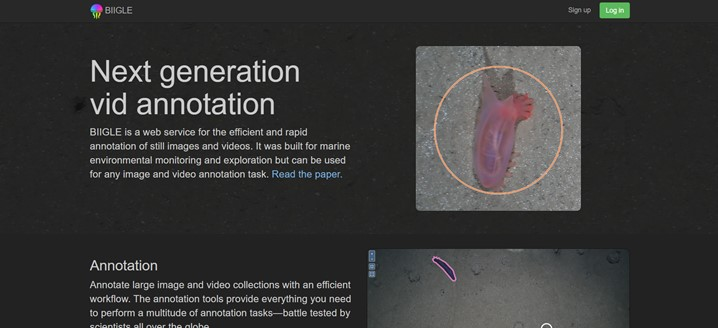
\includegraphics{/images/1.jpg}

Happy annotating!

\hypertarget{setting-up-on-biigle}{%
\section{Setting up on BIIGLE}\label{setting-up-on-biigle}}

Getting set up on BIIGLE (and other annotation softwares) first requires
that you host your imagery data, there are three options for this: via
BIIGLE (upload files on homepage); local instances and remote volumes.
See the BIIGLE manual for more details. Many institutes use a
cloud-based storage solution to host their remote volumes. This is not
the same as a google drive or equivalent where you might store or share
data. It is a formal repository that enables your images to each have a
unique URL. There are many types of cloud-based storage solutions that
you may wish to consider, key ones we are aware of include Amazon Web
Services (AWS), and Microsoft Azure. Each uses its own terminology to
refer to its storage `containers'. AWS calls its containers `Buckets',
Microsoft Azure calls them `Blobs'; they are the same thing.

Below we describe the process for setting up and working with AWS. We
invite others to contribute similar text for other cloud-storage
options.

\hypertarget{how-to-get-set-up-with-an-amazon-web-services-remote-server}{%
\subsection{How to get set up with an Amazon Web Services remote
server}\label{how-to-get-set-up-with-an-amazon-web-services-remote-server}}

Create an Amazon Web Services account.

On the AWS management console type ``S3'' into the find services search
box.

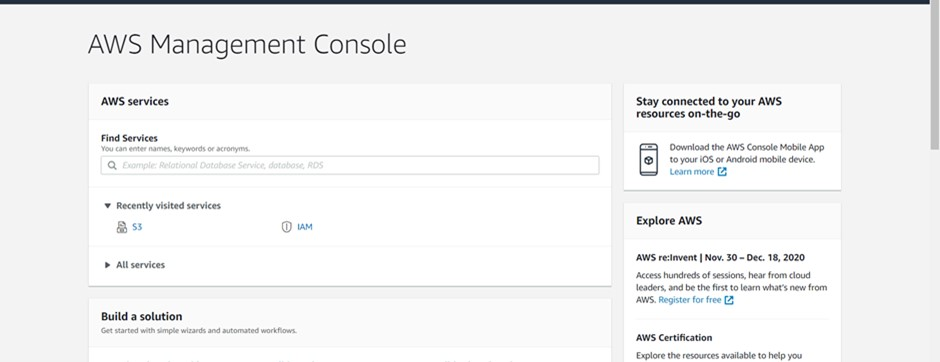
\includegraphics{/images/2.jpg}

Select ``S3''

Before you can upload data to Amazon S3, you must create a bucket in one
of the AWS regions to store your data.

Click on ``create bucket''

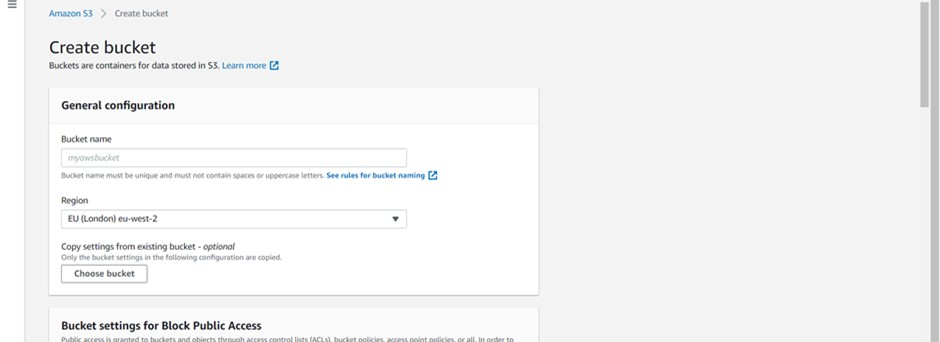
\includegraphics{/images/3.jpg}

Name your bucket in a sensible way. BIIGLE recommends you use their
personal random string generator {[}available here
https://biigle.de/manual/tutorials/volumes/remote-volumes{]} to do this
as this is hard to guess and keeps your data safer. But you can use
whatever name you like.

Select your nearest region

Uncheck the ``Block all public access'' box as BIIGLE needs to see your
folder.

Leave all other settings as default and click on ``create bucket''

Once you have created your bucket, click on it to take you to this
screen

\hypertarget{enabling-others-to-access-your-s3-aws-bucket-when-working-in-a-team}{%
\subsubsection{Enabling others to access your S3 AWS bucket when working
in a
team}\label{enabling-others-to-access-your-s3-aws-bucket-when-working-in-a-team}}

\hypertarget{formatting-your-data-for-use-in-biigle}{%
\subsection{Formatting your data for use in
BIIGLE}\label{formatting-your-data-for-use-in-biigle}}

\hypertarget{converting-video-file-to-upload-to-biigle}{%
\subsection{Converting video file to upload to
BIIGLE}\label{converting-video-file-to-upload-to-biigle}}

\hypertarget{recommendations-for-the-file-structure-of-your-bucket-and-file-naming-conventions}{%
\subsection{Recommendations for the file structure of your bucket and
file-naming
conventions}\label{recommendations-for-the-file-structure-of-your-bucket-and-file-naming-conventions}}

\hypertarget{setting-up-projects-and-volumes-in-biigle}{%
\section{Setting up projects and volumes in
BIIGLE}\label{setting-up-projects-and-volumes-in-biigle}}

\hypertarget{recommendations-for-project-volume-structuring-in-biigle}{%
\subsection{Recommendations for project / volume structuring in
BIIGLE}\label{recommendations-for-project-volume-structuring-in-biigle}}

\hypertarget{make-label-trees}{%
\subsection{Make label trees}\label{make-label-trees}}

\hypertarget{to-use-a-publicly-accessible-standard-tree}{%
\subsubsection{To use a publicly accessible (standard)
tree}\label{to-use-a-publicly-accessible-standard-tree}}

\hypertarget{creating-your-own-tree-from-scratch}{%
\subsubsection{Creating your own tree from
scratch}\label{creating-your-own-tree-from-scratch}}

\hypertarget{attaching-a-label-tree-to-your-project}{%
\subsection{Attaching a label tree to your
project}\label{attaching-a-label-tree-to-your-project}}

\hypertarget{make-annotations}{%
\section{Make annotations}\label{make-annotations}}

\hypertarget{image-annotation}{%
\subsection{Image annotation}\label{image-annotation}}

\hypertarget{video-annotation}{%
\subsection{Video annotation}\label{video-annotation}}

\hypertarget{setting-an-annotation-session}{%
\subsection{Setting an annotation
session}\label{setting-an-annotation-session}}

\hypertarget{quality-control-and-the-largo-tool}{%
\section{Quality control and the largo
tool}\label{quality-control-and-the-largo-tool}}

\hypertarget{suggested-best-practice-in-annotation}{%
\subsection{Suggested best practice in
annotation}\label{suggested-best-practice-in-annotation}}

\hypertarget{downloading-data-and-reformatting}{%
\section{Downloading data and
reformatting}\label{downloading-data-and-reformatting}}

\hypertarget{get-and-use-a-report}{%
\subsection{Get and use a report}\label{get-and-use-a-report}}

\hypertarget{image-annotation-report---csv-variant}{%
\subsubsection{Image annotation report - CSV
variant}\label{image-annotation-report---csv-variant}}

\hypertarget{using-the-biigle-api}{%
\section{Using the BIIGLE API}\label{using-the-biigle-api}}

\hypertarget{intro-to-biigles-application-programming-interface}{%
\subsection{Intro to BIIGLE's Application Programming
Interface}\label{intro-to-biigles-application-programming-interface}}

\hypertarget{basic-requests}{%
\subsection{Basic requests}\label{basic-requests}}

\hypertarget{requesting-a-biigle-report}{%
\subsubsection{Requesting a BIIGLE
report}\label{requesting-a-biigle-report}}

\hypertarget{requesting-the-id-numbers-of-biigle-objects}{%
\subsubsection{Requesting the ID numbers of BIIGLE
objects}\label{requesting-the-id-numbers-of-biigle-objects}}

\hypertarget{using-the-api-with-r-and-python}{%
\subsection{Using the API with R and
Python}\label{using-the-api-with-r-and-python}}

\hypertarget{accessing-label-tree-information}{%
\subsubsection{Accessing label tree
information}\label{accessing-label-tree-information}}

\hypertarget{uploading-annotations-to-biigle}{%
\subsection{Uploading annotations to
BIIGLE}\label{uploading-annotations-to-biigle}}

\hypertarget{exporting-biigle-files-for-use-in-yolo}{%
\section{Exporting BIIGLE files for use in
YOLO}\label{exporting-biigle-files-for-use-in-yolo}}

\hypertarget{future-updates-to-this-manual}{%
\section{Future updates to this
manual}\label{future-updates-to-this-manual}}



\end{document}
